\documentclass[aspectratio=169,11pt]{beamer}
\usetheme{Madrid}
\usecolortheme{default}
\setbeamertemplate{navigation symbols}{}
\setbeamertemplate{bibliography item}[text]
\usepackage{booktabs}
\usepackage{tabularx}
\usepackage{pgfplots}
\pgfplotsset{compat=1.17}
\usetikzlibrary{positioning,arrows.meta}

\title[Where to Enforce Coordination]{Where Should Coordination Be Enforced\\in Multi-Agent Software Engineering?}
\subtitle{Weekly Research Progress}
\author{Chiharu Tomimori}
\institute{Institute of Science Tokyo}
\date{\today}

% Full citation shown at the bottom of each paper slide
\newcommand{\papercite}[1]{%
  \vfill
  \begin{beamercolorbox}[wd=\textwidth,sep=3pt]{block body}
    \tiny #1
  \end{beamercolorbox}}

\newcommand{\yes}{\textcolor{green!50!black}{\checkmark}}
\newcommand{\no}{\textcolor{red!70!black}{$\times$}}

\tikzset{
  box/.style={draw, rounded corners, fill=blue!8, minimum height=0.9cm,
               text width=2.2cm, align=center, font=\footnotesize},
  hl/.style={box, fill=orange!20},
  arr/.style={-{Stealth[length=2mm]}, thick}
}

\begin{document}

% ---------------------------------------------------------------
\begin{frame}
  \titlepage
\end{frame}

% ---------------------------------------------------------------
\begin{frame}{This Week at a Glance}
  \centering
  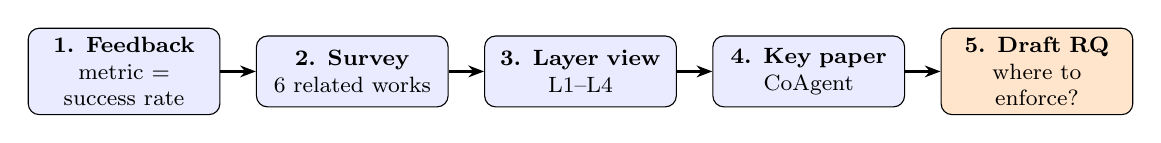
\begin{tikzpicture}[node distance=0.45cm]
    \node[box] (f) {\textbf{1. Feedback}\\metric = success rate};
    \node[box, right=of f] (s) {\textbf{2. Survey}\\6 related works};
    \node[box, right=of s] (l) {\textbf{3. Layer view}\\L1--L4};
    \node[box, right=of l] (k) {\textbf{4. Key paper}\\CoAgent};
    \node[hl, right=of k] (q) {\textbf{5. Draft RQ}\\where to enforce?};
    \draw[arr] (f) -- (s);
    \draw[arr] (s) -- (l);
    \draw[arr] (l) -- (k);
    \draw[arr] (k) -- (q);
  \end{tikzpicture}

  \vspace{1.2em}
  \small
  \begin{tabular}{ll}
    \toprule
    Done this week & Output \\
    \midrule
    Fixed the primary metric & Task success rate (hidden tests pass) \\
    Surveyed related work & CooperBench, CAID, PASC, NP-Bench, CoAgent, position paper \\
    Organized the landscape & Four coordination layers (L1--L4) \\
    Read CoAgent in depth & Strengths, limits, publication status \\
    Narrowed the question & Same protocol, different layers \\
    \bottomrule
  \end{tabular}
\end{frame}

% ---------------------------------------------------------------
\section{Problem}
\begin{frame}{Problem Setting}
  \centering
  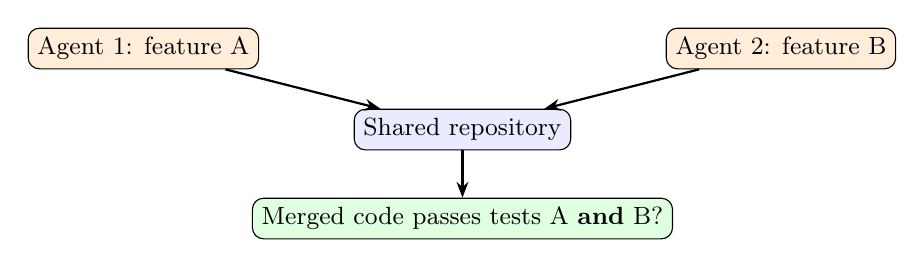
\begin{tikzpicture}[node distance=0.6cm and 1.4cm, every node/.style={font=\small}]
    \node[draw, rounded corners, fill=blue!8] (repo) {Shared repository};
    \node[draw, rounded corners, fill=orange!15, above left=0.5cm and 1.2cm of repo] (a1) {Agent 1: feature A};
    \node[draw, rounded corners, fill=orange!15, above right=0.5cm and 1.2cm of repo] (a2) {Agent 2: feature B};
    \node[draw, rounded corners, fill=green!12, below=0.6cm of repo] (t) {Merged code passes tests A \textbf{and} B?};
    \draw[arr] (a1) -- (repo);
    \draw[arr] (a2) -- (repo);
    \draw[arr] (repo) -- (t);
  \end{tikzpicture}

  \vspace{1em}
  \begin{itemize}
    \item Agents = \textbf{concurrent writers} on shared state
    \item Success = merged result passes \textbf{all} tests
  \end{itemize}
\end{frame}

% ---------------------------------------------------------------
\section{Related Work}
\begin{frame}{CooperBench: Can Two Agents Work as a Team?}
  \centering
  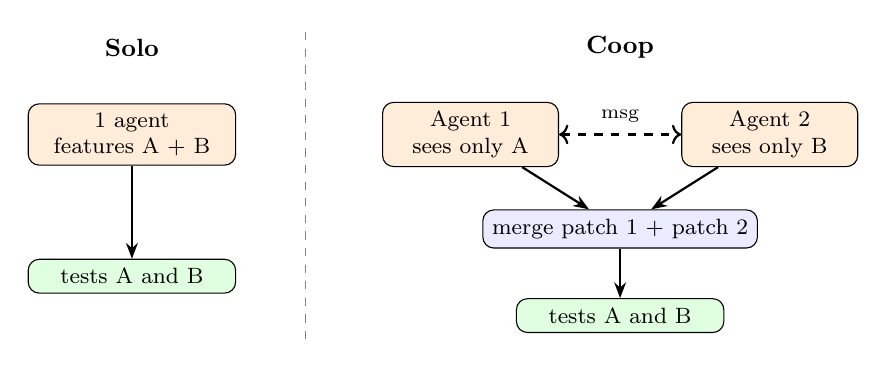
\begin{tikzpicture}[every node/.style={font=\footnotesize}]
    % solo
    \node[font=\small\bfseries] at (-3.6,2.3) {Solo};
    \node[draw, rounded corners, fill=orange!15, text width=2.4cm, align=center] (s) at (-3.6,1.2) {1 agent\\features A + B};
    \node[draw, rounded corners, fill=green!12, text width=2.4cm, align=center] (st) at (-3.6,-0.6) {tests A and B};
    \draw[arr] (s) -- (st);
    % coop
    \node[font=\small\bfseries] at (2.6,2.3) {Coop};
    \node[draw, rounded corners, fill=orange!15, text width=2.0cm, align=center] (c1) at (0.7,1.2) {Agent 1\\sees only A};
    \node[draw, rounded corners, fill=orange!15, text width=2.0cm, align=center] (c2) at (4.5,1.2) {Agent 2\\sees only B};
    \draw[<->, dashed, thick] (c1) -- node[above=3pt, font=\scriptsize, fill=white, inner sep=1pt]{msg} (c2);
    \node[draw, rounded corners, fill=blue!8] (m) at (2.6,0.0) {merge patch 1 + patch 2};
    \node[draw, rounded corners, fill=green!12, text width=2.4cm, align=center] (ct) at (2.6,-1.1) {tests A and B};
    \draw[arr] (c1) -- (m); \draw[arr] (c2) -- (m); \draw[arr] (m) -- (ct);
    \draw[gray, dashed] (-1.4,2.5) -- (-1.4,-1.5);
  \end{tikzpicture}

  \vspace{0.6em}
  \small
  \begin{tabular}{ll}
    Tasks & 652 feature pairs, 12 repos, 4 languages \\
    Built to conflict & features touch the same code \\
    Coordination & prompt + messaging tool only (no enforcement) \\
  \end{tabular}
  \papercite{A. Khatua, H. Zhu, P. Tran, A. Prabhudesai, F. Sadrieh, J. K. Lieberwirth, X. Yu, Y. Fu, M. J. Ryan, J. Pei, D. Yang. ``CooperBench: Why Coding Agents Cannot be Your Teammates Yet.'' \textit{Conference on Language Modeling (COLM)}, 2026. arXiv:2601.13295.}
\end{frame}

% ---------------------------------------------------------------
\begin{frame}{CooperBench: Results}
  \centering\small Two agents: $\sim$25\% success (GPT-5, Claude Sonnet 4.5), about \textbf{half of solo}. Messaging reduces merge conflicts but not failures.\\[4pt]
  \begin{columns}[T]
    \begin{column}{0.52\textwidth}
      \centering\footnotesize\textbf{Failure symptoms (\% of failures)}\\[2pt]
      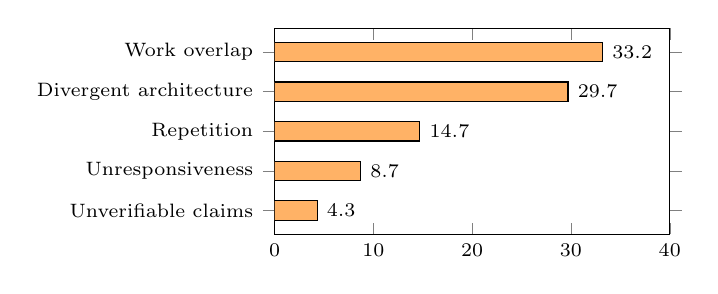
\begin{tikzpicture}
        \begin{axis}[xbar, width=6.6cm, height=4.2cm,
            xmin=0, xmax=40, bar width=7pt,
            symbolic y coords={Unverifiable claims,Unresponsiveness,Repetition,Divergent architecture,Work overlap},
            ytick=data, yticklabel style={font=\scriptsize},
            xticklabel style={font=\scriptsize},
            nodes near coords, nodes near coords style={font=\scriptsize},
            enlarge y limits=0.15]
          \addplot[fill=orange!60] coordinates {(4.3,Unverifiable claims) (8.7,Unresponsiveness) (14.7,Repetition) (29.7,Divergent architecture) (33.2,Work overlap)};
        \end{axis}
      \end{tikzpicture}
    \end{column}
    \begin{column}{0.46\textwidth}
      \centering\footnotesize\textbf{Success vs.\ number of agents (46 tasks)}\\[2pt]
      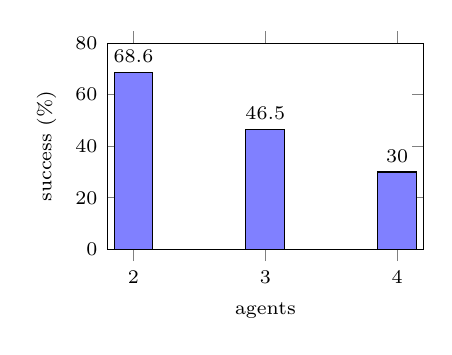
\begin{tikzpicture}
        \begin{axis}[ybar, width=5.6cm, height=4.2cm,
            ymin=0, ymax=80, bar width=14pt,
            symbolic x coords={2,3,4}, xtick=data,
            xlabel={agents}, ylabel={success (\%)},
            label style={font=\scriptsize}, ticklabel style={font=\scriptsize},
            nodes near coords, nodes near coords style={font=\scriptsize}]
          \addplot[fill=blue!50] coordinates {(2,68.6) (3,46.5) (4,30.0)};
        \end{axis}
      \end{tikzpicture}
    \end{column}
  \end{columns}
  \papercite{A. Khatua, H. Zhu, P. Tran, A. Prabhudesai, F. Sadrieh, J. K. Lieberwirth, X. Yu, Y. Fu, M. J. Ryan, J. Pei, D. Yang. ``CooperBench: Why Coding Agents Cannot be Your Teammates Yet.'' \textit{Conference on Language Modeling (COLM)}, 2026. arXiv:2601.13295.}
\end{frame}

% ---------------------------------------------------------------
\begin{frame}{Closest Work: CAID --- Branch and Merge}
  \centering
  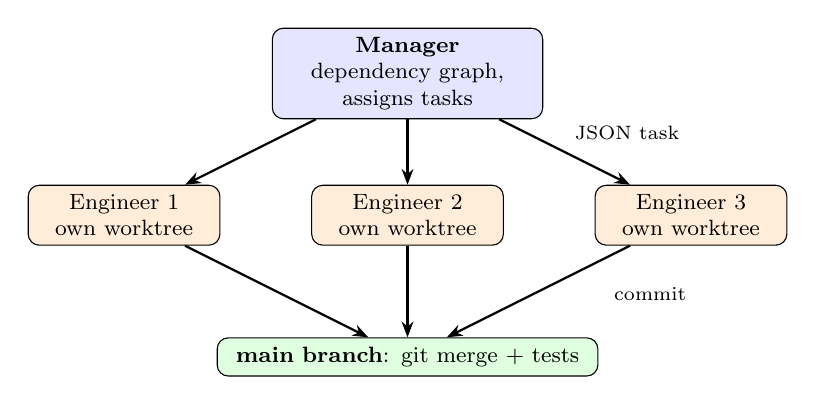
\begin{tikzpicture}[every node/.style={font=\footnotesize}]
    \node[draw, rounded corners, fill=blue!10, text width=3.2cm, align=center] (mgr) at (0,2.2) {\textbf{Manager}\\dependency graph,\\assigns tasks};
    \node[draw, rounded corners, fill=orange!15, text width=2.2cm, align=center] (e1) at (-3.6,0.4) {Engineer 1\\own worktree};
    \node[draw, rounded corners, fill=orange!15, text width=2.2cm, align=center] (e2) at (0,0.4) {Engineer 2\\own worktree};
    \node[draw, rounded corners, fill=orange!15, text width=2.2cm, align=center] (e3) at (3.6,0.4) {Engineer 3\\own worktree};
    \node[draw, rounded corners, fill=green!12, text width=4.6cm, align=center] (main) at (0,-1.4) {\textbf{main branch}: git merge + tests};
    \foreach \e in {e1,e2,e3} {\draw[arr] (mgr) -- (\e); \draw[arr] (\e) -- node[right, font=\scriptsize]{} (main);}
    \node[font=\scriptsize, right] at (2.5,-0.6) {commit};
    \node[font=\scriptsize, right] at (2.0,1.45) {JSON task};
  \end{tikzpicture}

  \vspace{0.5em}
  \small Parallel edits never touch each other's files directly; conflicts surface at merge time.
  \papercite{J. Geng, G. Neubig. ``Effective Strategies for Asynchronous Software Engineering Agents.'' arXiv:2603.21489, 2026 (preprint).}
\end{frame}

% ---------------------------------------------------------------
\begin{frame}{CAID: Results}
  \begin{columns}[T]
    \begin{column}{0.50\textwidth}
      \centering\footnotesize\textbf{Main result: higher score, higher cost}\\[4pt]
      \small
      \begin{tabular}{llcc}
        \toprule
        & & Single & CAID \\
        \midrule
        Commit0-Lite & score & 53.1 & \textbf{59.1} \\
                     & cost (\$) & 1.9 & 8.1 \\
                     & time (s) & 693 & 1583 \\
        \midrule
        PaperBench & score & 57.2 & \textbf{63.3} \\
                   & cost (\$) & 3.3 & 6.5 \\
                   & time (s) & 1804 & 2080 \\
        \bottomrule
      \end{tabular}\\[2pt]
      {\scriptsize Claude Sonnet 4.5; 4 engineers (Commit0), 2 (PaperBench)}
    \end{column}
    \begin{column}{0.48\textwidth}
      \centering\footnotesize\textbf{Ablation: how to isolate}\\[2pt]
      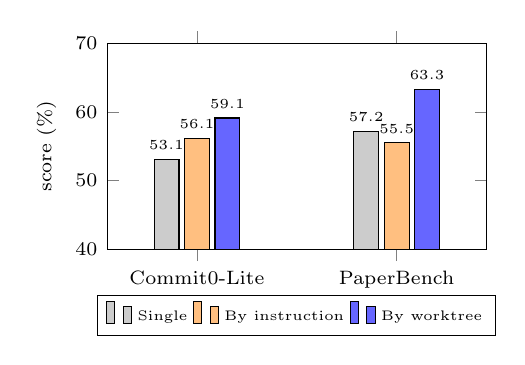
\begin{tikzpicture}
        \begin{axis}[ybar, width=6.4cm, height=4.2cm,
            ymin=40, ymax=70, bar width=9pt,
            symbolic x coords={Commit0-Lite,PaperBench}, xtick=data,
            ylabel={score (\%)}, label style={font=\scriptsize},
            ticklabel style={font=\scriptsize},
            enlarge x limits=0.45,
            legend style={font=\tiny, at={(0.5,-0.22)}, anchor=north, legend columns=3},
            nodes near coords, nodes near coords style={font=\tiny}]
          \addplot[fill=gray!40] coordinates {(Commit0-Lite,53.1) (PaperBench,57.2)};
          \addplot[fill=orange!50] coordinates {(Commit0-Lite,56.1) (PaperBench,55.5)};
          \addplot[fill=blue!60] coordinates {(Commit0-Lite,59.1) (PaperBench,63.3)};
          \legend{Single, By instruction, By worktree}
        \end{axis}
      \end{tikzpicture}
    \end{column}
  \end{columns}
  \vspace{0.2em}
  \footnotesize Limitation: with 8 engineers, two got the same file $\Rightarrow$ 92.1\% $\to$ 44.3\% on \texttt{simpy}.
  \papercite{J. Geng, G. Neubig. ``Effective Strategies for Asynchronous Software Engineering Agents.'' arXiv:2603.21489, 2026 (preprint).}
\end{frame}

% ---------------------------------------------------------------
\begin{frame}{Existing Work Coordinates at Different Layers}
  \small
  \begin{tabularx}{\textwidth}{l X l c}
    \toprule
    Layer & Mechanism & Example & Writes enforced? \\
    \midrule
    L1 Instruction & ``Do not touch others' files'' in the prompt & CooperBench coop [1] & \no \\
    L2 Advisory tool & Claim / scope tools the agent may ignore & NP-Bench [2] & \no \\
    L3 Runtime & Middleware blocks or reorders actions & CoAgent [3] & \yes \\
    L4 Workspace / VCS & Separate worktrees, merge with tests & CAID [4] & \yes \\
    \bottomrule
  \end{tabularx}
  \vspace{0.6em}

  \footnotesize NP-Bench lists enforced scopes as future work. PASC [5] (shared tree) sees co-edits rise from 16.8\% to 53.0\% (2 $\to$ 5 agents).
  \papercite{[1] Khatua et al., COLM 2026, arXiv:2601.13295. \;
  [2] S. Muku, ``Verifying Coordination in Parallel Coding Agents: NP-Bench and a Scheduling Planner,'' arXiv:2610.07261, 2026. \;
  [3] H. Lyu et al., arXiv:2606.15376, 2026. \;
  [4] J. Geng, G. Neubig, arXiv:2603.21489, 2026. \;
  [5] H. \"Ozayt\"urk, F. Buzluca, ``Coordinating Agents on a Shared Git Workspace: An Empirical Study of Action-Space Observation for Agentic Software Engineering,'' \textit{ESEM 2026}, LIPIcs vol.~394, 18:1--18:20. doi:10.4230/LIPIcs.ESEM.2026.18.}
\end{frame}

% ---------------------------------------------------------------
\section{Key Paper: CoAgent}
\begin{frame}{Key Paper: CoAgent --- The Runtime Informs, the Agent Repairs}
  \small\textbf{Problem}: agent B builds a canary on an image agent A is fixing $\Rightarrow$ final state matches \textbf{no serial order}
  \vspace{0.8em}

  \centering
  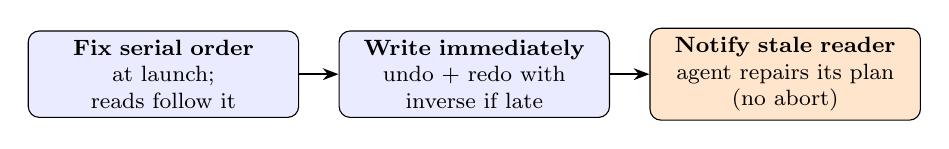
\begin{tikzpicture}[node distance=0.5cm]
    \node[box, text width=3.2cm] (o) {\textbf{Fix serial order}\\at launch;\\reads follow it};
    \node[box, text width=3.2cm, right=of o] (w) {\textbf{Write immediately}\\undo + redo with\\inverse if late};
    \node[hl, text width=3.2cm, right=of w] (n) {\textbf{Notify stale reader}\\agent repairs its plan\\(no abort)};
    \draw[arr] (o) -- (w);
    \draw[arr] (w) -- (n);
  \end{tikzpicture}

  \vspace{0.8em}
  \small
  \begin{tabular}{lll}
    \toprule
    & 2PL & OCC \\
    \midrule
    Problem with LLM agents & locks held during inference & abort wastes inference \\
    \bottomrule
  \end{tabular}
  \papercite{H. Lyu, D. Zhang, M. Wu, X. Wei, H. Chen. ``CoAgent: Concurrency Control for Multi-Agent Systems.'' arXiv:2606.15376, 2026 (preprint; no peer-reviewed version found as of Oct.\ 2026).}
\end{frame}

% ---------------------------------------------------------------
\begin{frame}{CoAgent: Results and Limitations}
  \centering\footnotesize\textbf{10 contended workloads, 2 agents (relative to serial execution)}\\[4pt]
  \small
  \begin{tabular}{lccl}
    \toprule
    Protocol & Speedup & Tokens & Note \\
    \midrule
    No coordination & $\sim$1.5$\times$ & -- & only 13\% of trials correct \\
    2PL & 1.04$\times$ & -- & 0.81 deadlocks / trial \\
    OCC & 0.93$\times$ & 1.83$\times$ & 0.95 aborts / trial \\
    \textbf{MTPO (proposed)} & \textbf{1.4$\times$} & \textbf{1.15$\times$} & correctness $\sim$5\% below serial \\
    \bottomrule
  \end{tabular}

  \vspace{0.8em}
  \footnotesize\textbf{Not covered by the evaluation}\\[3pt]
  \begin{tabular}{ccccc}
    \toprule
    Coding / git tasks & Prompt-only baseline & $>$2 agents & $>$1 model & Free-form bash \\
    \midrule
    \no & \no & \no & \no & \no \\
    \bottomrule
  \end{tabular}
  \papercite{H. Lyu, D. Zhang, M. Wu, X. Wei, H. Chen. ``CoAgent: Concurrency Control for Multi-Agent Systems.'' arXiv:2606.15376, 2026 (preprint).}
\end{frame}

% ---------------------------------------------------------------
\section{Research Question}
\begin{frame}{Gap and Draft Research Question}
  \small
  \begin{tabular}{l l c}
    \toprule
    Study & What is compared & Same protocol across layers? \\
    \midrule
    CoAgent [3] & Protocols inside L3 & \no \\
    CAID [4] & Isolation: L1 vs.\ L4 & partly \\
    NP-Bench [2] & Planning vs.\ detection, L2 only & \no \\
    Position paper [6] & Argument only, no experiments & \no \\
    \bottomrule
  \end{tabular}

  \vspace{1em}
  \begin{block}{Research question (draft)}
    At which layer should a coordination protocol (e.g., scope ownership) be enforced to maximize task success rate?
  \end{block}
  \papercite{[2] S. Muku, arXiv:2610.07261, 2026. \; [3] H. Lyu et al., arXiv:2606.15376, 2026. \; [4] J. Geng, G. Neubig, arXiv:2603.21489, 2026. \;
  [6] X. Yang, L. Li, Z. Ji, T. J. Zhang, W. Jiang. ``Position: Multi-Agent Systems Should Prioritize Concurrency Control.'' \textit{ICML 2026}. arXiv:2608.18092.}
\end{frame}

% ---------------------------------------------------------------
\begin{frame}{Same Protocol, Different Layers: An Example}
  \small\textbf{Protocol (fixed):} ``Agent 1 owns \texttt{a.py}; Agent 2 owns \texttt{b.py}. Edit only what you own.''\\[6pt]
  \centering
  \begin{tabularx}{\textwidth}{l X X c}
    \toprule
    Layer & How the rule is delivered & Agent 1 tries to edit \texttt{b.py} & Enforced? \\
    \midrule
    L1 Instruction & Written in the prompt & Edit succeeds & \no \\
    L2 Advisory tool & \texttt{claim(b.py)} says ``owned by Agent 2'' & Edit still succeeds & \no \\
    L3 Runtime & \texttt{b.py} is read-only for Agent 1 & \texttt{Permission denied} & \yes \\
    L4 Workspace & Own worktree; merge rejects out-of-scope files & Edit kept locally, rejected at merge & \yes~(late) \\
    \bottomrule
  \end{tabularx}

  \vspace{0.6em}
  \small Same rule, same owner map, same model and tasks --- only \textbf{who guarantees the rule} changes.
\end{frame}

% ---------------------------------------------------------------
\begin{frame}{Planned Experiment: Change Only the Layer}
  \centering
  \small
  \begin{tabular}{lll}
    \toprule
    Condition & Layer & Role \\
    \midrule
    Solo (1 agent, both features) & -- & reference \\
    Coop & L1 & existing \\
    Team mode (advisory claims) & L2 & existing \\
    \textbf{Enforced scopes (file permissions)} & \textbf{L3} & \textbf{proposed} \\
    Worktree + merge (CAID-style) & L4 & reference \\
    \bottomrule
  \end{tabular}

  \vspace{1em}
  \begin{tabular}{ll}
    Fixed & protocol, model, tasks, step budget \\
    Benchmark & CooperBench (gold patches conflict in 76.5\% of pairs) \\
    Primary metric & success rate (both features' tests pass) \\
    Secondary & out-of-scope writes, stale-read failures \\
  \end{tabular}
\end{frame}

% ---------------------------------------------------------------
\begin{frame}{Risks}
  \centering
  \small
  \begin{tabularx}{\textwidth}{l X}
    \toprule
    Risk & Mitigation \\
    \midrule
    One agent does all the work (serial collapse) & Report parallelism and ``rescued by one agent'' cases \\
    Stale reads not fixed by write partitioning & Count stale-read failures separately \\
    Blocked agents waste budget & Fix the denial message across runs \\
    Benchmark changed after the paper & Pin one commit of CooperBench \\
    Overlap with AgentRoom, ATM (2026 preprints) & Read them next week \\
    \bottomrule
  \end{tabularx}
\end{frame}

% ---------------------------------------------------------------
\begin{frame}{Next Week}
  \begin{enumerate}
    \item Run a small CooperBench pilot (10 pairs): solo / coop / team
    \item Classify the failures (write conflict, semantic conflict, stale read, capability)
    \item Count how often agents write outside their claims in team mode
    \item Read AgentRoom and ATM to check overlap
  \end{enumerate}
\end{frame}

% ---------------------------------------------------------------
\begin{frame}{Summary}
  \begin{itemize}
    \item Coordinating coding agents lose about \textbf{half} of their success
    \item Existing systems coordinate at \textbf{different layers}
    \item No study we found compares \textbf{the same protocol across layers}
  \end{itemize}
  \vspace{1em}
  \begin{block}{Takeaway}
    The question is not \emph{which protocol}, but \emph{where to enforce it}.
  \end{block}
\end{frame}

% ---------------------------------------------------------------
\begin{frame}[allowframebreaks]{References}
  \footnotesize
  \begin{thebibliography}{9}
    \bibitem{cooper} A. Khatua, H. Zhu, P. Tran, A. Prabhudesai, F. Sadrieh, J. K. Lieberwirth, X. Yu, Y. Fu, M. J. Ryan, J. Pei, D. Yang. CooperBench: Why Coding Agents Cannot be Your Teammates Yet. \textit{COLM}, 2026. arXiv:2601.13295.
    \bibitem{np} S. Muku. Verifying Coordination in Parallel Coding Agents: NP-Bench and a Scheduling Planner. arXiv:2610.07261, 2026.
    \bibitem{coagent} H. Lyu, D. Zhang, M. Wu, X. Wei, H. Chen. CoAgent: Concurrency Control for Multi-Agent Systems. arXiv:2606.15376, 2026.
    \bibitem{caid} J. Geng, G. Neubig. Effective Strategies for Asynchronous Software Engineering Agents. arXiv:2603.21489, 2026.
    \bibitem{pasc} H. \"Ozayt\"urk, F. Buzluca. Coordinating Agents on a Shared Git Workspace: An Empirical Study of Action-Space Observation for Agentic Software Engineering. \textit{ESEM}, LIPIcs vol.~394, 18:1--18:20, 2026. doi:10.4230/LIPIcs.ESEM.2026.18.
    \bibitem{pos} X. Yang, L. Li, Z. Ji, T. J. Zhang, W. Jiang. Position: Multi-Agent Systems Should Prioritize Concurrency Control. \textit{ICML}, 2026. arXiv:2608.18092.
  \end{thebibliography}
\end{frame}

\end{document}
